\documentclass[tikz,border=6pt]{standalone}
\usepackage{tikz}
\usetikzlibrary{arrows.meta,shapes.geometric}
\definecolor{navy}{RGB}{53,92,125}

\begin{document}
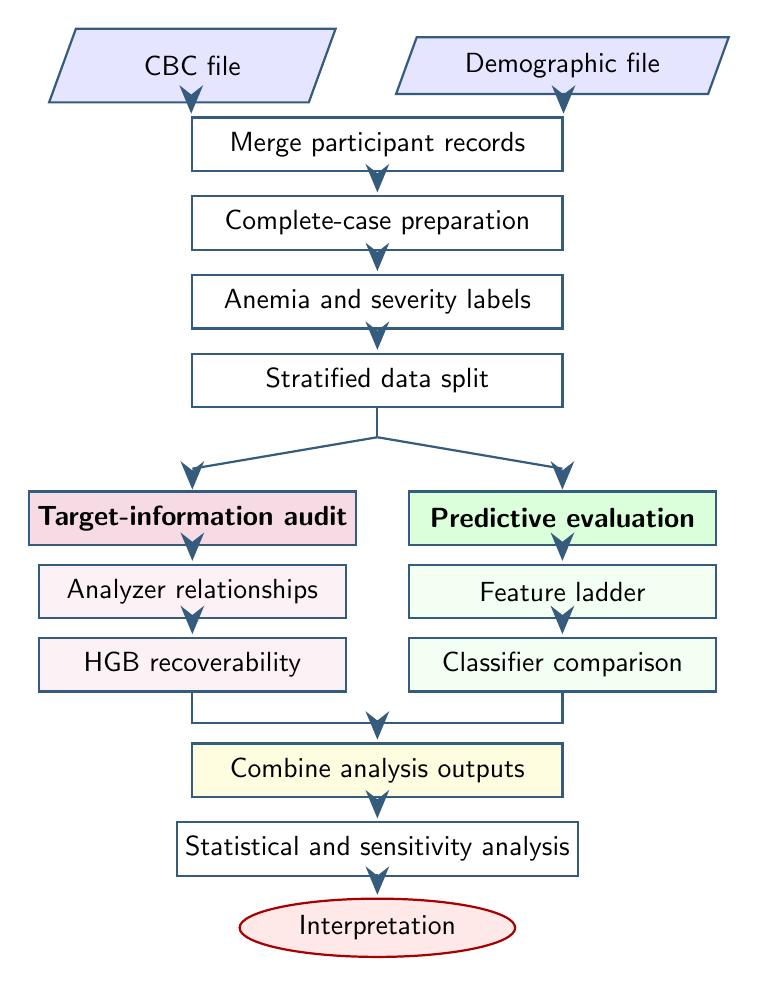
\begin{tikzpicture}[
  font=\sffamily,
  >={Stealth[length=3.6mm,width=3.0mm]},
  input/.style={draw=navy, fill=blue!10, trapezium,
    trapezium left angle=70, trapezium right angle=110,
    align=center, minimum width=3.65cm, minimum height=0.72cm,
    inner sep=3pt, line width=0.8pt},
  process/.style={draw=navy, fill=white, rectangle,
    align=center, minimum width=4.7cm, minimum height=0.68cm,
    inner sep=3pt, line width=0.8pt},
  heading/.style={draw=navy, rectangle, align=center,
    minimum width=3.9cm, minimum height=0.68cm,
    inner sep=3pt, line width=0.8pt, font=\sffamily\bfseries},
  task/.style={draw=navy, rectangle, align=center,
    minimum width=3.9cm, minimum height=0.68cm,
    inner sep=3pt, line width=0.8pt},
  output/.style={draw=red!65!black, fill=red!9, ellipse,
    align=center, minimum width=3.5cm, minimum height=0.68cm,
    inner sep=3pt, line width=0.8pt},
  arrow/.style={->, draw=navy, line width=0.8pt,
    shorten >=1pt, shorten <=1pt},
  line/.style={draw=navy, line width=0.8pt}
]

% Inputs and common preparation
\node[input] (cbc) at (-2.35,0) {CBC file};
\node[input] (demo) at (2.35,0) {Demographic file};
\node[process] (merge) at (0,-1.0) {Merge participant records};
\node[process] (cohort) at (0,-2.0) {Complete-case preparation};
\node[process] (labels) at (0,-3.0) {Anemia and severity labels};
\node[process] (split) at (0,-4.0) {Stratified data split};

\coordinate (cbc_drop) at (-2.35,-0.5);
\coordinate (demo_drop) at (2.35,-0.5);
\draw[arrow] (cbc.south) -- (cbc_drop) -| (merge.north west);
\draw[arrow] (demo.south) -- (demo_drop) -| (merge.north east);
\draw[arrow] (merge.south) -- (cohort.north);
\draw[arrow] (cohort.south) -- (labels.north);
\draw[arrow] (labels.south) -- (split.north);

% Clean fork: one junction line, two outgoing arrows
\coordinate (fork) at (0,-4.72);
\draw[line] (split.south) -- (fork);
\draw[line] (fork) -- (-2.35,-5.12);
\draw[arrow] (-2.35,-5.12) -- (-2.35,-5.42);
\draw[line] (fork) -- (2.35,-5.12);
\draw[arrow] (2.35,-5.12) -- (2.35,-5.42);

% Two aligned analysis branches
\node[heading, fill=purple!14] (audit) at (-2.35,-5.75) {Target-information audit};
\node[task, fill=purple!5] (identity) at (-2.35,-6.68) {Analyzer relationships};
\node[task, fill=purple!5] (recovery) at (-2.35,-7.61) {HGB recoverability};
\draw[arrow] (audit.south) -- (identity.north);
\draw[arrow] (identity.south) -- (recovery.north);

\node[heading, fill=green!14] (prediction) at (2.35,-5.75) {Predictive evaluation};
\node[task, fill=green!5] (ladder) at (2.35,-6.68) {Feature ladder};
\node[task, fill=green!5] (models) at (2.35,-7.61) {Classifier comparison};
\draw[arrow] (prediction.south) -- (ladder.north);
\draw[arrow] (ladder.south) -- (models.north);

% Clean join: incoming lines meet, then one outgoing arrow
\coordinate (join) at (0,-8.35);
\draw[line] (recovery.south) -- (-2.35,-8.35) -- (join);
\draw[line] (models.south) -- (2.35,-8.35) -- (join);
\node[process, fill=yellow!12] (combine) at (0,-8.95) {Combine analysis outputs};
\draw[arrow] (join) -- (combine.north);

\node[process] (statistics) at (0,-9.95) {Statistical and sensitivity analysis};
\node[output] (interpretation) at (0,-10.95) {Interpretation};
\draw[arrow] (combine.south) -- (statistics.north);
\draw[arrow] (statistics.south) -- (interpretation.north);

\end{tikzpicture}
\end{document}
